\item \textbf{{[}JPJC/PRELIM/9597/2019/P2/Q6{]} }

A reservation form used for booking JP Hotel rooms is shown:
\begin{center}
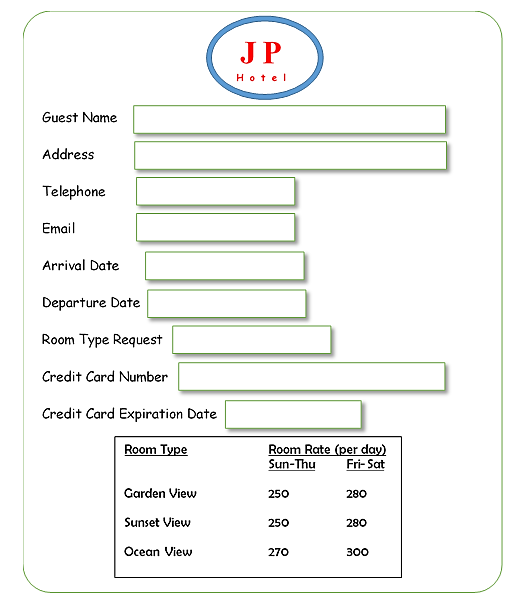
\includegraphics[width=0.5\paperwidth]{C:/Users/Admin/Desktop/Github/question_bank/LyX/static/img/9597-JPJC-2019-P2-Q6-1}
\par\end{center}

There are three room types available and the room rates are higher
for arrival on Fridays and Saturdays. A normalised database solution
is designed to store data for the hotel using a number of tables.
\begin{enumerate}
\item Draw an E-R diagram that shows these tables and the relationships
between them. \hfill{}{[}4{]}
\item Using standard notation, write the table descriptions of the tables
in part \textbf{(a)}. \hfill{} {[}6{]}
\end{enumerate}
To book a room in JP Hotel, the guest can fill in the hotel reservation
form with details specified on the form. After the form is submitted,
the credit card number and its expiration date are validated. The
guest will be notified with a message if the credit card number is
invalid. If the credit card number is valid, details of the guests
will be stored in a file. The room type requested by the guest will
then be checked for availability. If room type requested by guest
is available, a confirmation letter will be sent to the guest. 
\begin{enumerate}
\item[(c)]  Draw a data flow diagram for the hotel reservation system. \hfill{}{[}8{]}
\item[(d)]  A hotel room accommodates two guests and also includes breakfast
for two. The hotel allows for an additional guest to stay in a room
booked for two guests at a charge of \$80. An extra bed may be requested
for the additional guest at a charge of \$20. Breakfast can also be
provided for the additional guest at \$20.
\begin{enumerate}
\item Create a decision table showing all the possible conditions and actions.
\hfill{} {[}4{]}
\item Simplify your decision table by removing redundancies. \hfill{} {[}2{]}
\end{enumerate}
\end{enumerate}